\documentclass{llncs}
\usepackage{fancyhdr, tabularx, verbatim, epsfig}
\usepackage{amssymb,psboxit}
\usepackage{rotating}
\usepackage{tabularx}
\newcommand{\PyTrilinos}{{\sc PyTrilinos}}
\newcommand{\Trilinos}{{Trilinos}}
\newcommand{\TrilinosTM}{Trilinos \copyright}
\newcommand{\trilinos}{{Trilinos}}
\newcommand{\ifpack}{{Ifpack}}
\newcommand{\aztecoo}{{AztecOO}}
\newcommand{\amesos}{{Amesos}}
\newcommand{\epetra}{{Epetra}}
\newcommand{\ml}{{ML}}
\newcommand{\mb}[1]{{\mathbf {#1} }}
\newcommand{\teuchos}{{Teuchos}}
\newcommand{\triutils}{{Triutils}}
\newcommand{\metis}{{METIS}}

\newtheorem{interface}{Interface}[section]

\begin{document}

\pagestyle{headings} 
\mainmatter              % start of the contributions

\title{\PyTrilinos: High-Performance Distributed-Memory Solvers for
       Python}

\author{Marzio Sala\inst{1} \and William F. Spotz\inst{2} \and 
  Michael A. Heroux\inst{2}}
\titlerunning{High-Performance Computing in Python}

\authorrunning{Marzio Sala et al.}   % abbreviated author list (for running head)
%
%%%% modified list of authors for the TOC (add the affiliations)
\tocauthor{Marzio Sala (ETH Zurich),
William F. Spotz (Sandia National Laboratories),
Michael A. Heroux (Sandia National Laboratories)}
%
\institute{Department of Computer Science, ETH Zurich, CH-8092 Zurich\\
\email{marzio@inf.ethz.ch},
\and
  Sandia National Laboratories, 
PO Box 5800 MS 1110, Albuquerque, NM 87185-1110\footnote{
  ASCI program and the DOE Office of Science MICS program at Sandia
National Laboratory.  Sandia is a multiprogram laboratory operated by
Sandia Corporation, a Lockheed Martin Company, for the United States
Department of Energy's National Nuclear Security Administration under
contract DE-AC04-94AL85000.}.}

\maketitle              % typeset the title of the contribution

\begin{abstract}
\PyTrilinos\ is a collection of Python modules targeting serial
and parallel sparse linear algebra, direct and iterative linear
solution techniques, domain decomposition and multilevel
preconditioners, nonlinear solvers and continuation algorithms. Also
included are a variety of related utility functions and classes,
including distributed I/O, coloring algorithms and matrix
generation. \PyTrilinos\ vector objects are integrated with the
popular NumPy module, gathering together a variety of
high-level distributed computing operations with serial vector
operations.

\PyTrilinos\ uses a hybrid development approach, with a front-end in Python,
and a back-end, computational engine in compiled libraries. As such,
\PyTrilinos\ makes it easy to
take advantage of both the flexibility and ease of use of Python, and the
efficiency of the underlying C++, C and FORTRAN numerical kernels.  The
presented numerical results show that, for many important problem classes, the
overhead required by the Python interpreter is negligible.
\end{abstract}

%-----------------------------------------------------------------------------
\section{Introduction}
\label{sec:intro}
%-----------------------------------------------------------------------------

The choice of the programming language for the development of
large-scale, high-performance numerical algorithms is often a thorny
issue. 
It is difficult for a single programming
language to simultaneously support ease-of-use, rapid development, and
optimized executables.  Indeed, the goals of efficiency and
flexibility often conflict.  The key observation to approaching this
problem is that the time-critical portion of code requiring a compiled
language is typically a small set of self-contained functions or
classes.  Therefore, one can adopt an interpreted (and possibly
interactive) language, without a big performance degradation, provided
there is a robust interface between the interpreted and compiled code.

This article describes a collection of numerical linear algebra and
solver libraries, called \PyTrilinos, built on top of the
Trilinos~\cite{Trilinos-Overview}
project.  The main goal of \PyTrilinos\ is to port to a scripting
language most of the Trilinos capabilities, for faster development of novel
numerical algorithms.

Among the available scripting languages, we decided to adopt Python.  Python
is an interpreted, interactive, object-oriented programming language, which
combines remarkable power with very clean syntax (it is often observed that
well-written Python code reads like pseudo code).  Perhaps most importantly,
it can be easily extended by using a variety of open source tools such as
SWIG~\cite{swig}, f2py or pyfort to create wrappers to modules written in C, C++ or
FORTRAN for all performance critical tasks.

\PyTrilinos\ adds
significant power to the interactive Python session by providing
high-level commands and classes for the creation and usage of serial
and distributed, dense and sparse linear algebra objects.  Using
\PyTrilinos, an interactive Python session becomes a powerful
data-processing and system-prototyping environment that can be used to
test, validate, use and extend serial and parallel numerical
algorithms.  In our opinion, Python naturally complements languages
like C, C++ and FORTRAN as opposed to competing with them.  Similarly,
\PyTrilinos\ complements Trilinos by offering interactive and rapid
development.

\smallskip

This paper is organized as follows. Section~\ref{sec:why} reports more details
on the choice of Python and the interface generator tool, SWIG~\cite{swig}.
Section~\ref{sec:multilevel} gives an overview of the structure of \PyTrilinos,
which closely reflects the structure of the Trilinos framework. The
organization of \PyTrilinos\ is briefly outlined in
Section~\ref{sec:organization}, while Section~\ref{sec:serial} describes the
strategies adopted in parallel environments. Comparisons with MATLAB and
Trilinos are reported in Section~\ref{sec:comparison_matlab}. Finally,
Section~\ref{sec:discussion} draws the conclusions.

%-----------------------------------------------------------------------------
\section{Why Python and SWIG}
\label{sec:why}
%-----------------------------------------------------------------------------

Python has emerged as an excellent choice for scientific computing
because of its simple syntax, ease of use, object-oriented support and
elegant multi-dimensional array arithmetic.  Its interpreted
evaluation allows it to serve as both the development language and the
command line environment in which to explore data.  Python also excels
as a ``glue'' language between a large and diverse collection of
software packages---a common need in the scientific arena.

The Simple Wrapper and Interface Generator (SWIG)~\cite{swig} is a
utility that facilitates access to C and C++ code from Python. SWIG
will automatically generate complete Python interfaces (and other
languages) for existing C and C++ code.  It also supports multiple
inheritance and flexible extensions of the generated Python
interfaces.  Using these features, we can construct Python classes
that derive from two or more disjoint classes and we can provide
custom methods in the Python interface that were not part of the
original C++ interface.

Python combines broad capabilities with very clean syntax.  It has
modules, namespaces, classes, exceptions, high-level dynamic data
types, automatic memory management that frees the user from most
hassles of memory allocation, and much more.  Python also has some
features that make it possible to write large programs, even though
it lacks most forms of compile-time checking: a program can be
constructed out of modules, each of which defines its own namespace.
Exception handling makes it possible to catch errors where required
without cluttering the code with error checking.

Python's development cycle is typically much shorter than that of
traditional tools.  In Python, there are no compile or link
steps---Python programs simply import modules at runtime and use the
objects they contain.  Because of this, Python programs run
immediately after changes are made.  Python integration tools make
it usable in hybrid, multi-component applications.  As a
consequence, systems can simultaneously utilize the strengths of
Python for rapid development, and of traditional languages such as C
for efficient execution.  This flexibility is crucial in realistic
development environments.

%-----------------------------------------------------------------------------
\section{Multilevel Organization of \PyTrilinos}
\label{sec:multilevel}
%-----------------------------------------------------------------------------

\PyTrilinos\ is designed as a modular multilevel framework, and it takes
advantage of several programming languages at different levels.  The key
component is {\bf Trilinos}~\cite{Trilinos-Overview}, a set of numerical
solver packages in active development at Sandia National Laboratories that
allows high-performance scalable linear algebra operations for large systems
of equations.  The source code of the
current Trilinos public release accounts for about 300,000 code lines, divided
in about 67,000 code lines for distributed linear algebra objects and
utilities, 20,000 code lines for direct solvers and interfaces to third-party
direct solvers, 128,000 code lines for multilevel preconditioners, and 76,000
code lines for other algebraic preconditioners and Krylov accelerators. This
count does not include BLAS, LAPACK, MPI, and several other libraries used by
Trilinos. This explains why a ``pure'' Python approach is of no interest;
instead, we generate interfaces between the language in which most of
Trilinos packages are written, C++, and Python.

Although C++/Python interfaces can be generated by hand, it is more convenient
to adopt code generators to automate the process. We have adopted {\bf SWIG},
the Simplified Wrapper and Interface Generator, which is a preprocessor that
turns ANSI C/C++ declarations into scripting language interfaces, and produces
a fully working Python extension module.

It is important to note that \PyTrilinos\ is well-connected to other scientific
projects developed within the Python community. Indeed, \PyTrilinos\ vectors
inherit from the {\bf NumPy} vector class. NumPy is
a well-established Python module to handle multi-dimensional arrays including
vectors and matrices.  A large number of scientific packages and tools have
been written in or wrapped for Python that utilize NumPy for representing
fundamental linear algebra objects.  By integrating with NumPy, \PyTrilinos\
also integrates with this sizeable collection of packages. It also adopts {\bf
Distutils}, a Python module with utilities aimed at the portable distribution
of both pure Python modules and compiled extension modules.  Distutils has
been a part of the standard Python distribution since Python version 2.2.

%-----------------------------------------------------------------------------
\section{\PyTrilinos\ Organization}
\label{sec:organization}
%-----------------------------------------------------------------------------

\PyTrilinos\ reflects the Trilinos organization by presenting a series
of {\sl modules}, each of which wraps a given Trilinos {\sl package},
where a package is an integral unit usually developed by a small team
of experts in a particular area.  Trilinos packages that support
namespaces have a Python submodule for each namespace.  Algorithmic
capabilities are defined within independent packages; packages can
easily interoperate since generic adaptors are available (in the form
of pure virtual classes) to define distributed vectors and matrices. The
modules currently included are briefly described below.

\smallskip

\noindent 
The first and most important \PyTrilinos\ module is {\bf
Epetra}~\cite{Epetra-Ref-Guide}, a collection of concrete classes to support
the construction and use of vectors, sparse distributed graphs, and dense and
distributed sparse matrices.  It provides serial, parallel and distributed
memory linear algebra objects.  Epetra supports double-precision floating
point data only, and uses BLAS and LAPACK where possible, and as a result has
good performance characteristics.  All the other \PyTrilinos\ modules depend on
Epetra. 

\smallskip

\noindent
{\bf EpetraExt} offers a variety of extension capabilities to
  the Epetra package, such as input/output and coloring algorithms.
  The I/O capabilities make it possible to read and write generic
  Epetra objects (like maps, matrices and vectors) or import and
  export data from and to other formats, such as MATLAB, the
  Harwell/Boeing or Matrix Market format, therefore
  accessing a large variety of well-recognized test cases for dense
  and sparse linear algebra.

\smallskip

\noindent
{\bf Galeri} allows the creation of several matrices, like the
  MATLAB's {\tt gallery} function, and it can be useful for examples
  and testing. 

\smallskip

\noindent
{\bf Amesos}~\cite{Amesos-Reference-Guide} contains a set of clear and consistent interfaces
  to the following third-party serial and parallel sparse direct
  solvers: UMFPACK,
  PARDISO, TAUCS, SuperLU
  and SuperLU\_DIST,
  DSCPACK, MUMPS, and
  ScaLAPACK.  As such,
  \PyTrilinos\ makes it possible to access state-of-the-art direct
  solver algorithms developed by groups of specialists, and written in
  different languages (C, FORTRAN77, FORTRAN90), in both serial and
  parallel environments.  By using Amesos, more than 350,000 code
  lines (without considering BLAS, LAPACK, and ScaLAPACK) can be
  easily accessed from any code based on Trilinos (and therefore
  \PyTrilinos).

\smallskip

\noindent
{\bf AztecOO}~\cite{Aztec} provides object-oriented access to
preconditioned Krylov accelerators, like CG, GMRES and several others, based
on the popular Aztec library.  One-level domain decomposition preconditioners
based on incomplete factorizations are available.

\smallskip

\noindent
{\bf IFPACK}~\cite{ifpack-guide} contains object-oriented algebraic preconditioners,
  compatible with Epetra and AztecOO.  It supports construction and
  use of parallel distributed memory preconditioners such as
  overlapping Schwarz domain decomposition with several local solvers.
  IFPACK can take advantage of SPARSKIT, a widely used
  software package.

\smallskip

\noindent
{\bf ML}~\cite{ml-guide} contains a set of multilevel preconditioners based on
  aggregation procedures for serial and vector problems compatible
  with Epetra and AztecOO.  ML can use the METIS and
  ParMETIS libraries to create the aggregates.  

\smallskip

\noindent
{\bf NOX} is a collection of nonlinear solver algorithms.  NOX
  is written at a high level with low level details such as data
  storage and residual computations left to the user.  This is
  facilitated by interface base classes which users can inherit from
  and define concrete methods for residual fills, Jacobian matrix
  computation, etc.  NOX also provides some concrete classes which
  interface to Epetra, LAPACK, PETSc and others.

\smallskip
\noindent
{\bf LOCA} is the library of continuation algorithms.  It is
  based on NOX and provides stepping algorithms for one or more
  nonlinear problem parameters.

\smallskip
\noindent
{\bf New\_Package} is a parallel ``Hello World'' code whose
  primary function is to serve as a template for Trilinos developers
  for how to establish package interoperability and apply standard
  utilities such as auto-tooling and
  automatic documentation to their own packages.  For the purposes of
  \PyTrilinos, it provides an example of how to wrap a Trilinos
  package.

%-----------------------------------------------------------------------------
\section{Serial and Parallel Environments}
\label{sec:serial}
%-----------------------------------------------------------------------------

Although testing and development of high-performance algorithms can be
done in serial environments, parallel environments still constitute
the most important field of application for most Trilinos algorithms.
However, Python itself does not provide any parallel support.  Because
of this, several projects have been developed independently to fill
the gap between Python and MPI. 
All of these projects allow the use of Python through the interactive
prompt, but additional overhead is introduced.  Also, none of these
projects define a well-recognized standard, since they are still under
active development.

The \PyTrilinos\ approach is somewhat complementary to the efforts of these
projects.  We decided to use a standard, out-of-the-box, Python
interpreter, then wrap only the very basics of MPI: MPI\_Init(),
MPI\_Finalize(), and MPI\_COMM\_WORLD.  By wrapping these three
objects, we can define an MPI-based Epetra communicator (derived from
the pure virtual class Epetra\_Comm class), on which all wrapped
Trilinos packages are already based.  This reflects the philosophy of
all the considered Trilinos packages, that have no explicit dependency
on MPI communicators, and accept the pure virtual class Epetra\_Comm
instead. 

The major disadvantage of our approach is that Python cannot be run
interactively if more than one processor is used.  Although all the
most important MPI calls are available through Epetra.Comm objects
(for example, the rank of a process is returned by method {\tt
  comm.MyPID()} and the number of processes involved in the
computation by method {\tt comm.NumProc()}), not all the functions
specified by the MPI forum are readily available through this object.
For example, at the moment there are no point-to-point communications,
or non-blocking functions (though they could be easily added in the
future).

In our opinion, these are only minor drawbacks, and the list of
advantages is much longer.  First, since all calls are handled by
Epetra, no major overhead occurs, other than that of parsing a Python
instruction.  Second, all \PyTrilinos\ modules that require direct MPI
calls can dynamically cast the Epetra.Comm object, retrieve the MPI
communicator object, then use direct C/C++ MPI calls.  As such, the
entire set of MPI functions is available to developers with no
additional overhead.  Third, a standard Python interpreter is used.
Finally, serial and parallel scripts can be identical, and \PyTrilinos\
scripts can be run in parallel from the shell in the typical way.

%-----------------------------------------------------------------------------
\section{Numerical Results}
\label{sec:comparison_matlab}
%-----------------------------------------------------------------------------

We now present some numerical results that compare the CPU time
required by \PyTrilinos\ and MATLAB 7.0 (R14) to create a  serial
sparse matrix.  The test creates a sparse diagonal matrix, setting one element
at a time.  The MATLAB code reads:
\begin{verbatim}
    A = spalloc(n, n, n);
    for i=1:n
      A(i,i) = 1;
    end
\end{verbatim}
while the \PyTrilinos\ code contains the instructions:
\begin{verbatim}
    A = Epetra.CrsMatrix(Epetra.Copy, Map, 1)
    for i in xrange(n):
      A.InsertGlobalValues(i, [1.0], [i])
    A.FillComplete()
\end{verbatim}
Clearly, other techniques exist to create in MATLAB and in
\PyTrilinos\ sparse diagonal matrices.  However, the presented example
is representative of several real applications, which often have the
need of setting the elements of a matrix one (or a few) at a time.
Numerical results for this test case are reported in
Table~\ref{tab:matlab_sparse}, left.  Even for mid-sized sparse matrices,
\PyTrilinos\ is much faster than MATLAB's built-in sparse matrix
capabilities.  Table~\ref{tab:matlab_sparse}, right, reports the CPU required
for a matrix-vector product.  The sparse matrices arise from a 5-pt
discretization of a Laplacian on a 2D Cartesian grid (as produced in
MATLAB by the command {\tt gallery('poisson', n)}).  Note that
\PyTrilinos\ is up to 50\% faster than MATLAB for this very important
computational kernel.

Since \PyTrilinos\ is intended largely for sparse matrices, these
results confirm the achievement of project goals compared to MATLAB,
especially because the set of algorithms available in \PyTrilinos\ to
handle and solve sparse linear systems is superior to that available
in MATLAB.

\begin{table}
  \begin{center}
    \begin{tabular}{|r|r@{.}l|r@{.}l|}
      \hline
      $n$ & \multicolumn{2}{c|}{MATLAB} &
      \multicolumn{2}{c|}{\PyTrilinos} \\
      \hline
      \hline
        1,000 &  0&00397 & 0&0059   \\
       10,000 &  0&449   & 0&060    \\
       50,000 & 11&05    & 0&313    \\
      100,000 & 50&98    & 0&603    \\
      \hline
    \end{tabular}
    \hspace*{3mm}
    \begin{tabular}{|r|r@{.}l|r@{.}l|}
      \hline
      $n$ & \multicolumn{2}{c|}{MATLAB} &
      \multicolumn{2}{c|}{\PyTrilinos} \\
      \hline
      \hline
         50 &  0&02  & 0&0053 \\
        100 &  0&110 & 0&0288 \\
        500 &  3&130 & 1&782  \\
      1,000 & 12&720 & 7&150  \\
      \hline
    \end{tabular}
    \vspace*{1mm}
    \caption{On the left, CPU time (in seconds) required by MATLAB and
      \PyTrilinos\ to set the elements of a sparse diagonal matrix of
      size $n$. On the right, CPU time (in seconds) required by MATLAB and
      \PyTrilinos\ to perform 100 matrix-vector products.  The sparse
      matrices, of size $n \times n$, correspond to a 5-pt
      discretization of a 2D Laplacian on a rectangular Cartesian
      grid.}
    \label{tab:matlab_sparse}
  \end{center}
\end{table}

\smallskip

We now report numerical comparisong for a matrix-vector product performed
in \PyTrilinos\ and in Trilinos, using the Epetra package. The results are given
in Figure~\ref{fig:time_parallel_matvec}.
Experiments were conducted on
a 16-node Linux/GCC/LAM-MPI cluster where each node has a single AMD
Athlon (Barton 2600) processor and the cluster has a dedicated Fast
Ethernet switch for inter-node communication.  The timing results show
that there is essentially no difference in timing results for either
version, and that parallel scalability is excellent, as it should be
for this type of problem.

\begin{figure}
  \begin{center}
    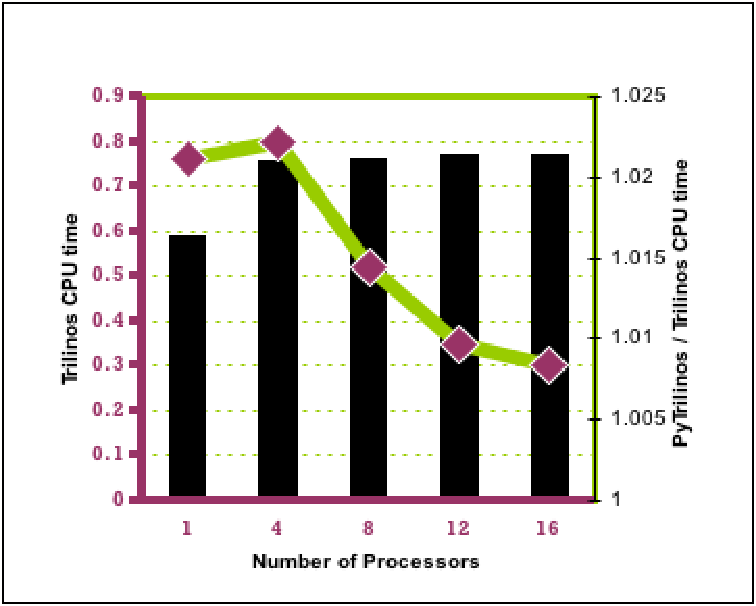
\includegraphics[width=6cm]{scalability-1k}
    \caption{Wall-clock time (in seconds) on 16-node Linux/GCC cluster.
      The bars report the time required by Trilinos (scale on the
      left), while the line reports the ratio between the time
      required by \PyTrilinos\ and the time required by Trilinos (scale
      on the right).}
    \label{fig:time_parallel_matvec}
  \end{center}
\end{figure}

%-----------------------------------------------------------------------------
\section{Conclusions}
\label{sec:discussion}
%-----------------------------------------------------------------------------

In this paper we have presented an overview of the
\PyTrilinos\ project, an effort to facilitate the design, integration
and ongoing support of Python access to a large collection of
mathematical software libraries.  \PyTrilinos\ provides a simple but
powerful rapid development environment, along with the integration
tools needed to apply it in realistic environments.  In our opinion,
the most significant impact of \PyTrilinos\ is in the following areas:

\begin{itemize}
%
\item {\bf Rapid Prototyping.}  Because Python is a simple language,
  coding is much faster than in other languages.  For example, its
  dynamic typing, built-in containers, and garbage collection
  eliminate much of the manual bookkeeping code typically required in
  languages like C or C++.  As most bookkeeping code is missing,
  Python programs are easier to understand and more closely reflect
  the actual problem they're intended to address.  Often, well-written
  Python code looks like pseudo code, and as such it is easier to
  write, read, and maintain.
%
\item {\bf Brevity.} Python codes can be short and concise.  Since
  things like type declaration, memory management, and common data
  structure implementations are absent, Python programs are typically
  a fraction of their C or C++ equivalents.  Brevity is also promoted
  by the object-oriented design of both \PyTrilinos\ and Trilinos
  itself.  Python scripts are short, generally with few jump
  statements, and therefore have good software metrics in terms of
  code coverage.
%
\item {\bf Modularity and Reusability.} Python allows the code to be organized in
  reusable, self-contained modules.  This also reflects the natural
  structure of Trilinos itself.  Since Python supports both procedural
  and object-oriented design, users can adopt their preferred way of
  writing code.
%
\item {\bf Explorative Computation.} Since Python is an interpreted
  and interactive scripting language, the user can undertake
  computations in an explorative and dynamic manner.  Intermediate
  results can be examined and taken into account before the next
  computational step, without the compile-link-run cycle typical of C
  or C++.
%
\item {\bf Integration.} Python was designed to be a ``glue'' language
  and \PyTrilinos\ relies on the ability to mix components written in
  different languages.  Python lends itself to experimental,
  interactive program development, and encourages developing systems
  incrementally by testing components in isolation and putting them
  together later.  By themselves, neither C nor Python is adequate to
  address typical development bottlenecks; together, they can do much
  more.  The model we are using splits the work effort into {\sl
    front-end} components that can benefit from Python's easy-of-use
  and {\sl back-end} modules that require the efficiency of compiled
  languages like C, C++, or FORTRAN.
%
\item {\bf Software Quality.} Software quality is of vital importance
  in the development of numerical libraries.  If the quality of the
  software used to produce a new computation is questionable, then the
  result must be treated with caution as well.  If, however, the
  quality of the software is high, it can reliably be made available
  to other research groups.

  Producing high quality software for state-of-the-art algorithms is a
  challenging goal.  Therefore, the production of high quality
  software requires a comprehensive set of testing programs.  A way to
  do that without influencing the rapid development of prototype code,
  is to write tests in Python.  By helping to detect defects,
  \PyTrilinos\ can become an important testing tool for Trilinos itself.
  (Clearly, \PyTrilinos\ tests require a bug-free interface between
  Trilinos and \PyTrilinos.) Using \PyTrilinos\ in the Trilinos test
  harness, one can experiment with the code to detect and manage
  dynamic errors, while static errors (like argument checking) must be
  detected by other types of testing.
%
\item {\bf Stability.} The only Python module on which
  \PyTrilinos\ depends is NumPy, for both serial and parallel
  applications.  Since NumPy is a well-supported and stable module,
  users can develop their applications based on \PyTrilinos\ with no
  need to change or update them in the near future.
%
\item {\bf Data Input.} All scientific applications require data to be
  passed into the code.  Typically, this data is read from one or more
  files and often the input logic becomes extensive in order to make
  the code more flexible.  In other words, the scientific code
  developers often find themselves implementing a rudimentary
  scripting language to control their application.  We have found that
  applications developed in Python avoid this distraction from more
  scientific work because the Python scripts themselves become
  high-level ``input files,'' complete with variable definitions,
  looping capabilities and every other Python feature.
\end{itemize}

\smallskip

Of course, Python (and by extension \PyTrilinos) is not the perfect
language or environment for all problems.  The most important problems
we have encountered are:

\begin{itemize}
%
\item {\bf Portability.} \PyTrilinos\ is developed concurrently on
  both Linux and Mac OS X, and it should port successfully to most
  other platforms where Trilinos, Python, NumPy and SWIG are
  available.  However, configuring Trilinos, and thus \PyTrilinos, for
  a new platform can be a non-trivial exercise.
%
\item {\bf Shared Libraries on Massively Parallel Computers.} Another
  problem is related to the shared library approach, the
  easiest way of integrating third-party libraries in Python.  Most
  massively parallel computers do not support shared libraries,
  making Python scripts unusable for very large scale
  computations.
%
\item {\bf Lack of Compile-time Checks.} In Python all checks must be
  performed at run-time.  Furthermore, Python does not support strong
  typing of variables, so user mistakes related to incorrect variable
  types can be a challenge to find and correct, where these types of
  mistakes would be caught quickly by a strongly-typed language and
  compiling system such as C++ and Java.
%
\item {\bf Performance Considerations.}  By using a Python wrapper, a
  performance penalty is introduced due to decoding of Python code,
  the execution of wrapped code, and returning the results in a
  Python-compliant format.  These tasks may require thousands of CPU
  cycles, therefore it is important to recognize this situation when
  it occurs.  The performance penalty is small if the C/C++ function
  does a lot of work.  Therefore, for rarely called functions, this
  penalty is negligible.  All performance critical kernels should be
  written in C, C++, or Fortran, and everything else can be in Python.
%
\item {\bf Management of C/C++ Arrays.} Although SWIG makes it easy to
  wrap Python's lists as C and C++ arrays (and vice-versa), this
  process still requires the programmer to define wrappers in the
  interface file, that converts the array into a list, or a list into
  an array.  Without an explicit wrapper, the proper handling of
  arrays can result in non-intuitive code, or memory leaks.
\end{itemize}

The most important feature of Python is its powerful but
simple programming environment designed for development speed and for
situations where the complexity of compiled languages can be a
liability.  Of course, Python enthusiasts will point out several other
strengths of the language; our aim was to show that Python can be
successfully used to develop and access state-of-the-art numerical
solver algorithms, in both serial and parallel environments.

We believe that \PyTrilinos\ is a unique effort. For the first time
a large number of high-performance algorithms for distributed sparse
linear algebra is easily available from a scripting language.  None
of the previously reported projects for scientific computing with
Python handles sparse and distributed matrices, or the diversity of
solver algorithms.  We hope that \PyTrilinos\ can help to make the
development cycle of high-performance numerical algorithms more
efficient and productive.

%-----------------------------------------------------------------------------%
\bibliographystyle{alpha}
\bibliography{paper}
%-----------------------------------------------------------------------------%

\end{document}
